\section{Linealización alrededor de los puntos de equilibrio}

\subsection*{Esquema conceptual}
El modelo de levitación magnética se analizó haciendo uso de principios elementales, de esta manera se obtuvo su dinámica no lineal. La variable de control es el voltaje del electroimán superior $u(t)$, y la variable controlada es la posición del disco $y(t)$.
\subsection*{Modelo no lineal}
El movimiento de todo sistema electromagnético lo componen: la ecuación mecánica descrita por la segunda ley de Newton que muestra la relación entre la posición de la masa y el conjunto de fuerzas que actúan sobre dicha masa; la ecuación electromecánica que describe la relación entre la tensión aplicada por el actuador, la posición del disco ferromagnético y la fuerza electromagnética sobre el mencionado disco; y finalmente la ecuación eléctrica que relaciona la tensión aplicada por el actuador con la corriente que circula por el electroimán.

\subsection*{Modelado en espacio de estados}
Si denotamos ${x}_{1}$ y ${x}_{2}$, respectivamente como posición y velocidad de la masa y se propone el cambio de variable:
\begin{align*} 
&x_{1}=  y_{(t)} \\ 
&\dot{x}_{1}=x_{2}
\end{align*}

La realización en espacio de estados para el caso inestable es:

\begin{align*}
    \begin{cases}
        \dot{x}_1 = x_2 \\
        \dot{x}_2 = \dfrac{u_{(t)}}{bm(a - x_1)^4} - \dfrac{c}{m}x_2 - g
    \end{cases}
\end{align*}

Donde  $u_{(t)}$ es el voltaje aplicado a las terminales de la bobina, $g$ es la aceleración de la gravedad, $c$ es el coeficiente de fricción, $m$ la masa del disco ferromagnético, $a$ y $b$ parámetros físicos. El problema que se pretende resolver es calcular el valor de $u_{(t)}$ para establecer la posición $x_{1}$ de la masa dada una referencia de posición.
Por otro lado, podemos expresar:
\begin{align*}
    \dot{x}_{1} &= f_{1}(t;x_{1};u) \\
    \dot{x}_{2} &= f_{2}(t;x_{2}; u)
\end{align*}

Finalmente, se define el vector de funciones como:
\begin{align*}
    \dot{x} = f(t,x, u) = 
    \begin{bmatrix}
    x_2 \\
    \dfrac{u_{(t)}}{bm(a - x_1)^4} - \dfrac{c}{m}x_2 - g
    \end{bmatrix}
\end{align*}

\begin{figure}[h]
    \centering
    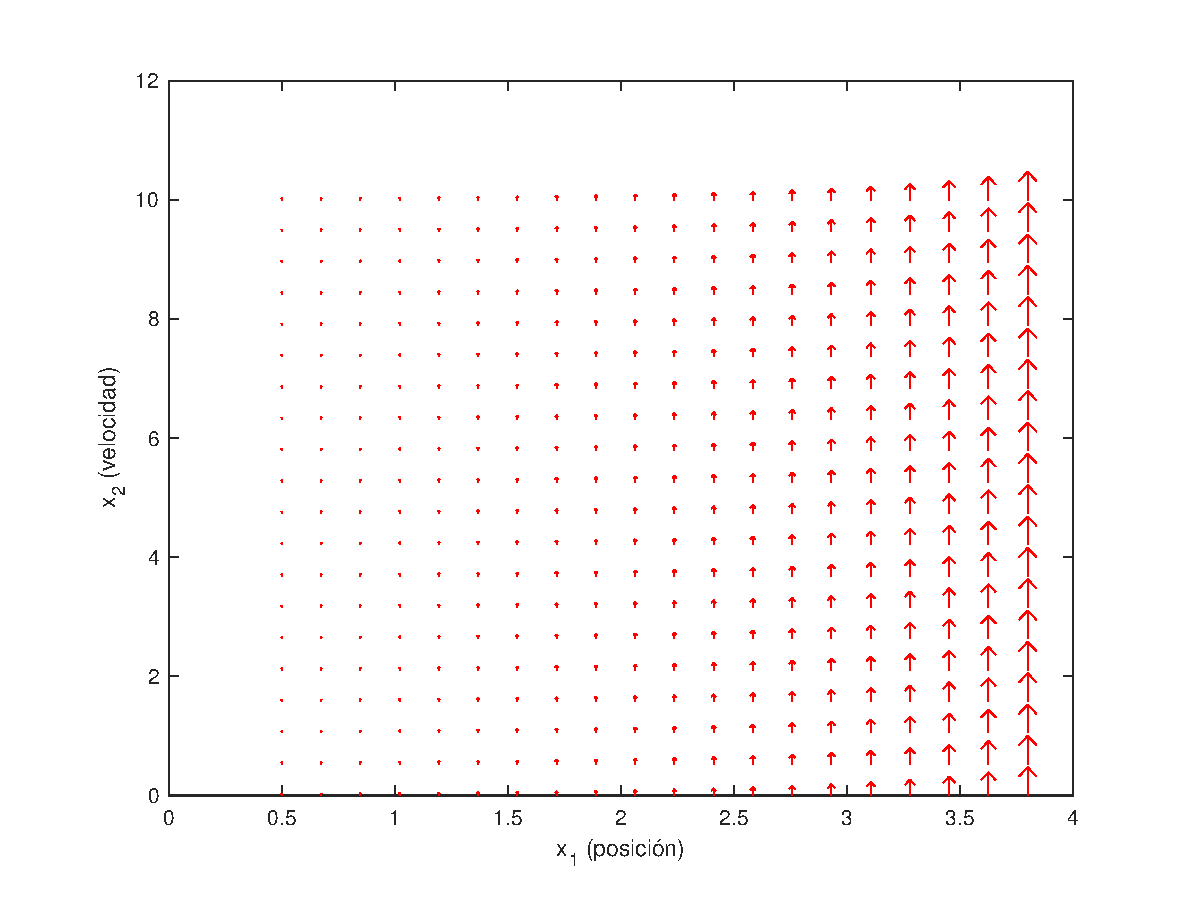
\includegraphics[width=0.5\textwidth]{images/chapter_1/phase_portrait.eps}
    \caption{Campo de vectores del sistema de levitación magnética.}
    \label{portrait_phase}
\end{figure}
Las trayectorias con formas incrementales muestran la solución
sin acción de control, lo que permite clasificar el sistema como no lineal, de tipo escape de tiempo finito.\cite{khalil1} 

\subsection*{Análisis del comportamiento cualitativo del sistema linealizado alrededor del punto de equilibrio}

Considerando que el sistema se encuentra en estado de equilibrio, o sea, para $\dot{x} = 0$:

\begin{align*}
    &\dot{x_{1}}=x_{2}=0\\
    &\dot{x_{2}}=\dfrac{u_{(t)}}{bm(a-x_{1})^4}- \dfrac{c}{m}x_{2} - g=0
\end{align*}

La solución del sistema de ecuaciones es:
\begin{align*}
    &x_{11}^{e}=a -{{\left(\dfrac{u_{e}}{b\,g\,m}\right)}}^{1/4}\\
\end{align*}

Se tiene que el valor de los puntos de equilibrio se puede determinar como: 
\begin{align*}
    &x_{1}^{e}=a -{{\left(\dfrac{u_{e}}{b\,g\,m}\right)}}^{1/4} \\
    &x^{e}_{2}=0
\end{align*}


Obtenemos las matrices jacobianas con respecto a los vectores de estado $x = 
\begin{bmatrix}
x_1 \\
x_2
\end{bmatrix}$ y el vector de entrada $u$ como:

\begin{align*}
    A = \dfrac{\partial f}{\partial x} 
    &=
    \renewcommand{\arraystretch}{3}
        \left[
            \begin{array}{cc}
                \dfrac{\partial \dot{x}_1}{\partial x_1} & \dfrac{\partial \dot{x}_1}{\partial x_2} \\
                \dfrac{\partial \dot{x}_2}{\partial x_1} & \dfrac{\partial \dot{x}_2}{\partial x_2}
            \end{array}
        \right]
    \renewcommand{\arraystretch}{4.0}\\[1ex]
    &= 
        \begin{bmatrix}
        0 & 1 \\[3ex]
        \dfrac{4u}{bm (a - x_{1})^5} & -\dfrac{c}{m}
    \end{bmatrix}_{\bigg|_{x_{1}=x_e, u=u_{e}}}
    \\[1ex]    
    &=
    \begin{bmatrix}
        0 & 1 \\[3ex]
        \dfrac{4u_{e}}{bm \left( a - \left( a - \left( \dfrac{u_{e}}{bgm} \right)^{1/4}\right) \right)^5} & -\dfrac{c}{m}
    \end{bmatrix} \\[1ex]
    &=
    \begin{bmatrix}
        0 & 1 \\[3ex]
        \dfrac{4u_{e}}{bm \left( \dfrac{u_{e}}{bgm} \right)^{5/4}} & -\dfrac{c}{m}
    \end{bmatrix}
\end{align*}


\begin{align*}
    B = \dfrac{\partial f}{\partial u} 
    &=
        \renewcommand{\arraystretch}{2.5}
        \left[
            \begin{array}{c}
                \dfrac{\partial \dot{x}_1}{\partial u} \\
                \dfrac{\partial \dot{x}_2}{\partial u}
            \end{array}
        \right]
        \renewcommand{\arraystretch}{2.5}\\[1ex]
     &=
        \begin{bmatrix}
            0 \\[2ex]
             \dfrac{1}{bm (a - x_{1})^4}
        \end{bmatrix}_{\bigg|_{x_{1}=x_e}}\\[1ex]  
   &=
        \begin{bmatrix}
            0 \\[2ex]
            \dfrac{1}{bm\left(a- \left( a -{{\left(\dfrac{1}{b\,g\,m}\right)}}^{1/4}\right)\right)^4}
        \end{bmatrix}\\[1ex]
    &= 
        \left[
            \begin{array}{c}0\\[2ex]
                \dfrac{1}{g}
            \end{array}
        \right]
\end{align*}

Finalmente:
\begin{equation*}
    \dot{q}=\left[\begin{array}{cc}
    0 & 1\\\\
\dfrac{4u_{e}}{bm \left( \dfrac{u_{e}}{bgm} \right)^{5/4}} & -\dfrac{c}{m}
\end{array}\right]q + 
\left[\begin{array}{c}0\\\\
\dfrac{1}{g}
\end{array}\right]u
\end{equation*}
%Concentrando la atención sobre el componente sin fuerza $Aq$, planteamos que el sistema es continuamente diferenciable sobre $\mathbb{R}^2$, por tanto es localmente Lipschitz, sin embargo, no es globalmente Lipschitz dado que $\frac{\partial f}{\partial x}$ no está uniformemente acotada en $\mathbb{R}^{2}$.

Por otro lado:
\begin{align*}
y &= \begin{bmatrix} 1 & 0 \end{bmatrix}q, \\
D &= 0
\end{align*}

Donde el estado $q \in Q \subset \mathbb{R}^2$, la entrada de control $u \in \mathbb{R}$, la salida regulada, $y \in \mathbb{R}$.

Aplicando la fórmula de la ecuación de transferencia:
\begin{align*}
G(s) &= C(sI - A)^{-1}B + D
\end{align*}
Si
\[
sI - A = 
\begin{bmatrix}
s & 0 \\
0 & s
\end{bmatrix}
-
\begin{bmatrix}
0 & 1 \\[2ex]
\dfrac{4u_{e}}{bm \left( \dfrac{u_{e}}{bgm} \right)^{5/4}} & -\dfrac{c}{m}
\end{bmatrix}
=
\begin{bmatrix}
s & -1 \\[2ex]
- \dfrac{4u_{e}}{bm \left( \dfrac{u_{e}}{bgm} \right)^{5/4}}  & s + \frac{c}{m} 
\end{bmatrix}
\]

Si se calcula \( \left| sI - A \right| \) entonces:

\begin{align*}
\left| sI - A \right| &= s \left( s + \frac{c}{m} \right) - \frac{4 u_{e}}{b m \left( \frac{u_{e}}{b g m} \right)^{5/4}} \\
                      &= s^2 + \frac{c}{m} s - \frac{4 u_{e}}{b m \left( \frac{u_{e}}{b g m} \right)^{5/4}}
\end{align*}

Ahora la adjunta de \( (sI - A) \) es:

\begin{equation*}
    \operatorname{adj}(sI - A) = 
    \begin{bmatrix}
    s + \dfrac{c}{m} & 1 \\[2ex]
    \dfrac{4u_{e}}{bm \left( \dfrac{u_{e}}{bgm} \right)^{5/4}} & s
    \end{bmatrix}
\end{equation*}


Entonces, la inversa de \( (sI - A) \) es:
\begin{equation*}
    \det(sI - A)^{-1} \cdot \operatorname{adj}(sI - A) = 
\dfrac{1}{s^2 + \dfrac{c}{m}s - \dfrac{4u_{e}}{bm \left( \dfrac{u_{e}}{bgm} \right)^{5/4}}} 
\begin{bmatrix}
s + \dfrac{c}{m} & 1 \\[2ex]
\dfrac{4u_{e}}{bm \left( \dfrac{u_{e}}{bgm} \right)^{5/4}} & s
\end{bmatrix}
\end{equation*}




Multiplicamos por $C$ y $B$ como:
\begin{align*}
    C(sI - A)^{-1}B 
        &=
        \begin{bmatrix} 1 & 0 \end{bmatrix} 
        \cdot 
        \left[ 
            \dfrac{1}{s^2 + \dfrac{c}{m}s - \dfrac{4u_{e}}{bm \left( \dfrac{u_{e}}{bgm} \right)^{5/4}}}
            \cdot 
           \begin{bmatrix}
                s + \dfrac{c}{m} & 1 \\[2ex]
                \dfrac{4u_{e}}{bm \left( \dfrac{u_{e}}{bgm} \right)^{5/4}} & s
           \end{bmatrix}
        \right]
        \cdot 
        \begin{bmatrix} 0 \\[2ex] \dfrac{1}{g} \end{bmatrix} \\[1em]
        &= 
            \dfrac{1}{s^2 + \dfrac{c}{m}s - \dfrac{4u_{e}}{bm \left( \dfrac{u_{e}}{bgm} \right)^{5/4}}} 
            \cdot
            \left[
                \begin{bmatrix} 1 & 0 \end{bmatrix}
                \cdot
               \begin{bmatrix}
                s + \dfrac{c}{m} & 1 \\[2ex]
                \dfrac{4u_{e}}{bm \left( \dfrac{u_{e}}{bgm} \right)^{5/4}} & s
               \end{bmatrix}
            \cdot
                \begin{bmatrix} 0 \\[2ex] \dfrac{1}{g} \end{bmatrix}
            \right] \\[1em]
        &= 
            \dfrac{1}{s^2 + \dfrac{c}{m}s - \dfrac{4u_{e}}{bm\left(\dfrac{u_{e}}{bgm}\right)^{5/4}}}
            \cdot 
            \left[
                \begin{bmatrix} s + \dfrac{c}{m} & 1 \end{bmatrix} 
                \cdot
                \begin{bmatrix} 0 \\[2ex]\dfrac{1}{g} \end{bmatrix}
            \right] \\[1em]
        &=  
            \frac{1}{g} 
            \cdot 
            \dfrac{1}{s^2 + \dfrac{c}{m}s - \dfrac{4u_{e}}{bm\left(\dfrac{u_{e}}{bgm}\right)^{5/4}}}
\end{align*}

Finalmente:
\begin{equation*}
    G_{(s)} = \frac{1}{g} \cdot \dfrac{1}{s^2 + \dfrac{c}{m}s - \dfrac{4u_{e}}{bm \left( \dfrac{u_{e}}{bgm} \right)^{5/4}}}
\end{equation*}

De igual manera:
\begin{equation*}
    G_{(s)} = \dfrac{K}{s^2 + \dfrac{c}{m}s - \dfrac{4u_{e}}{bm \left( \dfrac{u_{e}}{bgm} \right)^{5/4}}}
\end{equation*}

Donde:
\begin{equation*}
    K = \frac{1}{g},
    \qquad 
    \omega_0 = \dfrac{4u_{e}}{bm \left( \dfrac{u_{e}}{bgm} \right)^{5/4}}, \qquad 
    \alpha = \frac{c}{m}
\end{equation*}

Entonces, los polos son las raíces de:
\begin{equation*}
   s^2 + \dfrac{c}{m}s -\dfrac{4u_{e}}{bm \left( \dfrac{u_{e}}{bgm} \right)^{5/4}} = 0 
\end{equation*}

Aplicando la fórmula general:
\begin{align*}
    s 
    &= 
        \dfrac{ 
            -\dfrac{c}{m} \pm 
            \sqrt{ 
                \left( \dfrac{c}{m} \right)^2 
                - 4 
                \cdot 
                \left( -\dfrac{4u_e}{bm \left( \dfrac{u_e}{bgm} \right)^{5/4}} \right)
            }
        }{2} \\[1ex]
    &= 
        \dfrac{ 
           - \dfrac{c}{m} \pm 
            \sqrt{ 
                \left( \dfrac{c}{m} \right)^2 
                + 16 
                \cdot 
                \left( \dfrac{u_e}{bm \left( \dfrac{u_e}{bgm} \right)^{5/4}} \right)
            }
        }{2}
\end{align*}


O de forma más clara:
\begin{equation*}
    s_{1,2} = \frac{-\alpha \pm \sqrt{\alpha^2 + 16\omega_0}}{2}
\end{equation*}

Al mommento del discriminante ser positivo y los polos tener la forma:

\begin{equation*}
    s_1 = \frac{-\alpha + \sqrt{\alpha^2 + 4\omega_0^2}}{2} > 0, \qquad
    s_2 = \frac{-\alpha - \sqrt{\alpha^2 + 4\omega_0^2}}{2} < 0
\end{equation*}

Podemos afirmar que se tienen dos polos reales, de signos contrarios; por tanto, el sistema es inestable, de fase no mínima.

Tomándose como punto de equilibrio $u_{e} = 3.4826$ y $x_{e} =
\begin{bmatrix}
-4 \\
0
\end{bmatrix}$, se tiene que el valor de los polos es de -23.5057 y 14.9427; por tanto, la representación del lugar de las raíces y el mapa de polos y ceros es de la siguiente manera: 

\newpage
\begin{figure}[!h]
  \centering
  \subfloat{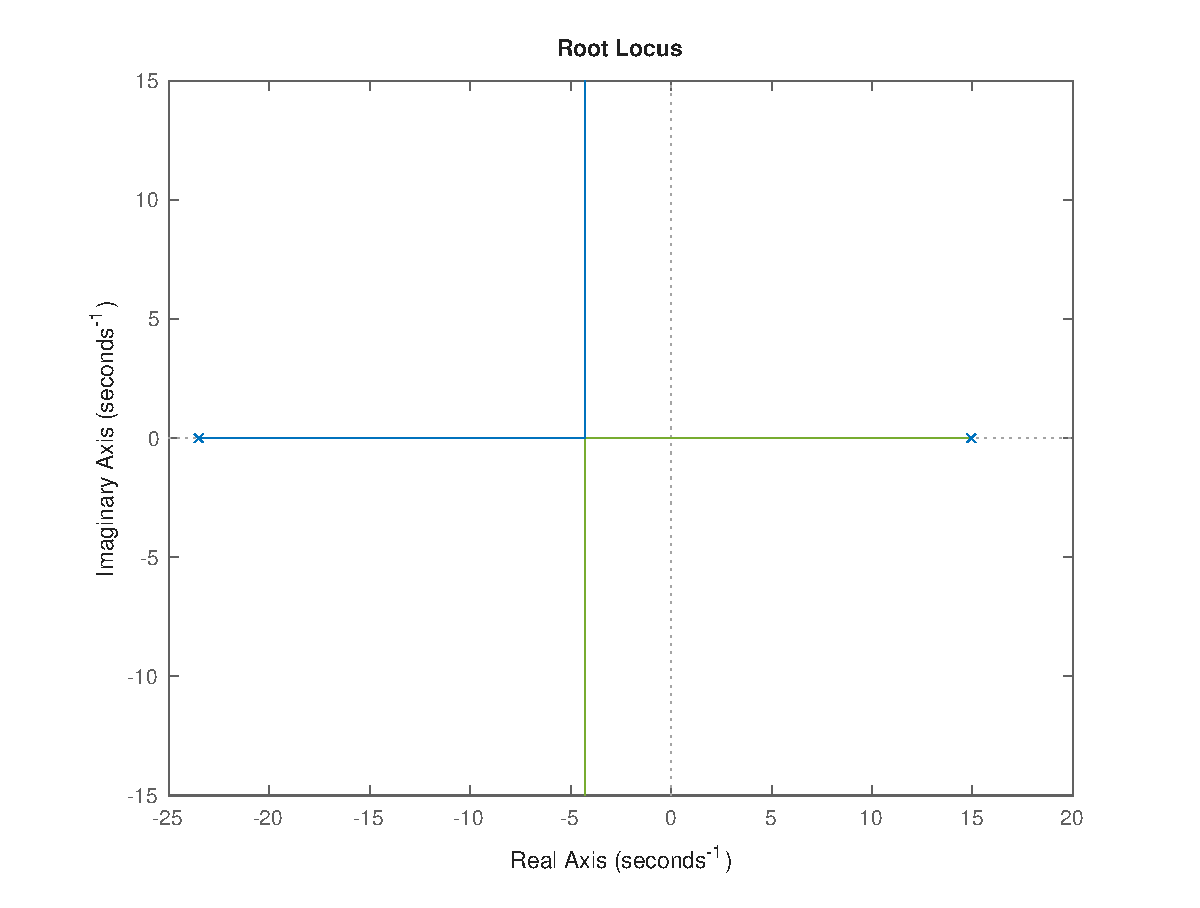
\includegraphics[width=0.5\linewidth]{images/chapter_1/root_locus.eps}}
  \subfloat{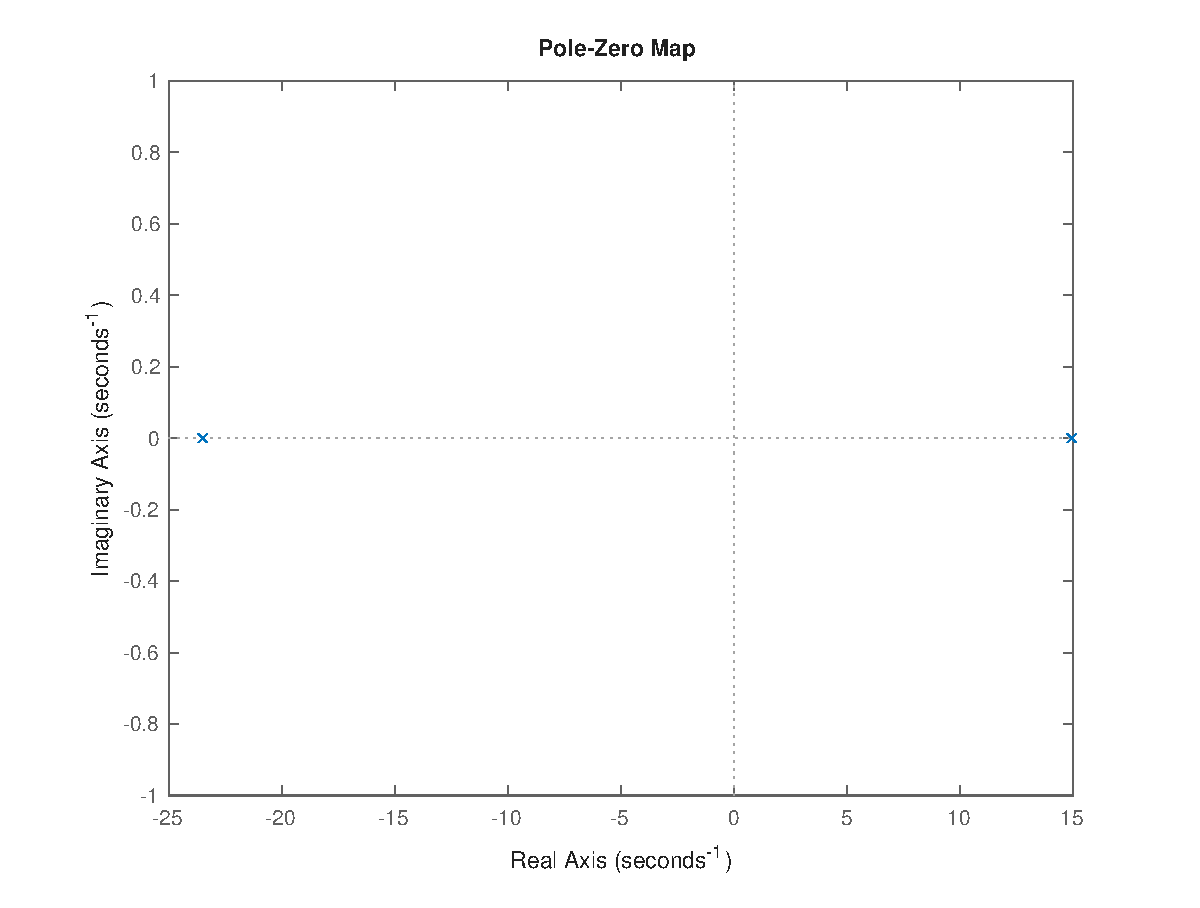
\includegraphics[width=0.5\linewidth]{images/chapter_1/pole_zero_map.eps}}
\end{figure}

Adicionalmente, al realizar el análisis de comportamiento cualitativo del sistema tenemos que $A$ es una matriz cuadrada que soporta operaciones de suma y multiplicación, cumple con el teorema de Cayley-Hamilton, y por tanto satisface su propia ecuación característica que se puede expresar como el polinomio característico:

\begin{equation*}
    p_{A}(\lambda) = \det(\lambda I - A)
\end{equation*}


Se construye $\lambda I - A$:

\begin{align*}
\lambda I - A
    &= 
    \begin{bmatrix}
        \lambda & 0 \\
        0 & \lambda
    \end{bmatrix}
    -
    \begin{bmatrix}
        0 & 1 \\[1ex]
       \dfrac{4u_{e}}{bm \left( \dfrac{u_{e}}{bgm} \right)^{5/4}} & -\dfrac{c}{m}
    \end{bmatrix} \\[2.0ex]
    &=
    \begin{bmatrix}
        \lambda & -1 \\[1ex]
        -\dfrac{4u_{e}}{bm \left( \dfrac{u_{e}}{bgm} \right)^{5/4}} & \lambda + \dfrac{c}{m}
    \end{bmatrix}
\end{align*}

Evaluando en el determinante se obtiene:
\begin{align*}
    \det(\lambda I - A)
    &= \begin{vmatrix}
        \lambda & -1 \\[1ex]
        -\dfrac{4u_{e}}{bm \left( \dfrac{u_{e}}{bgm} \right)^{5/4}} & \lambda + \dfrac{c}{m}
    \end{vmatrix} \\[2.0ex]
    &= \lambda\left(\lambda + \dfrac{c}{m} \right) - \dfrac{4u_{e}}{bm \left( \dfrac{u_{e}}{bgm} \right)^{5/4}} 
\end{align*}

Por lo tanto, el polinomio característico del sistema linealizado está dado por:

\begin{equation*}
 \lambda^2 + \dfrac{c}{m}\,\lambda-\dfrac{4u_{e}}{bm \left( \dfrac{u_{e}}{bgm} \right)^{5/4}}=0 
\end{equation*}

Con soluciones:
\begin{equation*}
    \lambda_{1,2} = 
    \dfrac{
        -\dfrac{c}{m} \pm 
        \sqrt{
            \left( \dfrac{c}{m} \right)^2 
            - 4 \cdot 
            \left( -\dfrac{4u_e}{bm \left( \dfrac{u_e}{bgm} \right)^{5/4}} \right)
        }
    }{2}
\end{equation*}

De igual manera, se puede hacer una simplificación semejante al resultado anterior, que resulta en base a la forma de los autovalores y sin pérdida de generalidad en que $\lambda_{2}<0<\lambda_{1}$;  por lo tanto,  el sistema  no lineal contiene múltiples puntos de equilibrio aislados de tipo silla, como se puede apreciar en el diagrama de fase en coordenadas modales.\cite{khalil2} 

\begin{figure}[h]
    \centering
    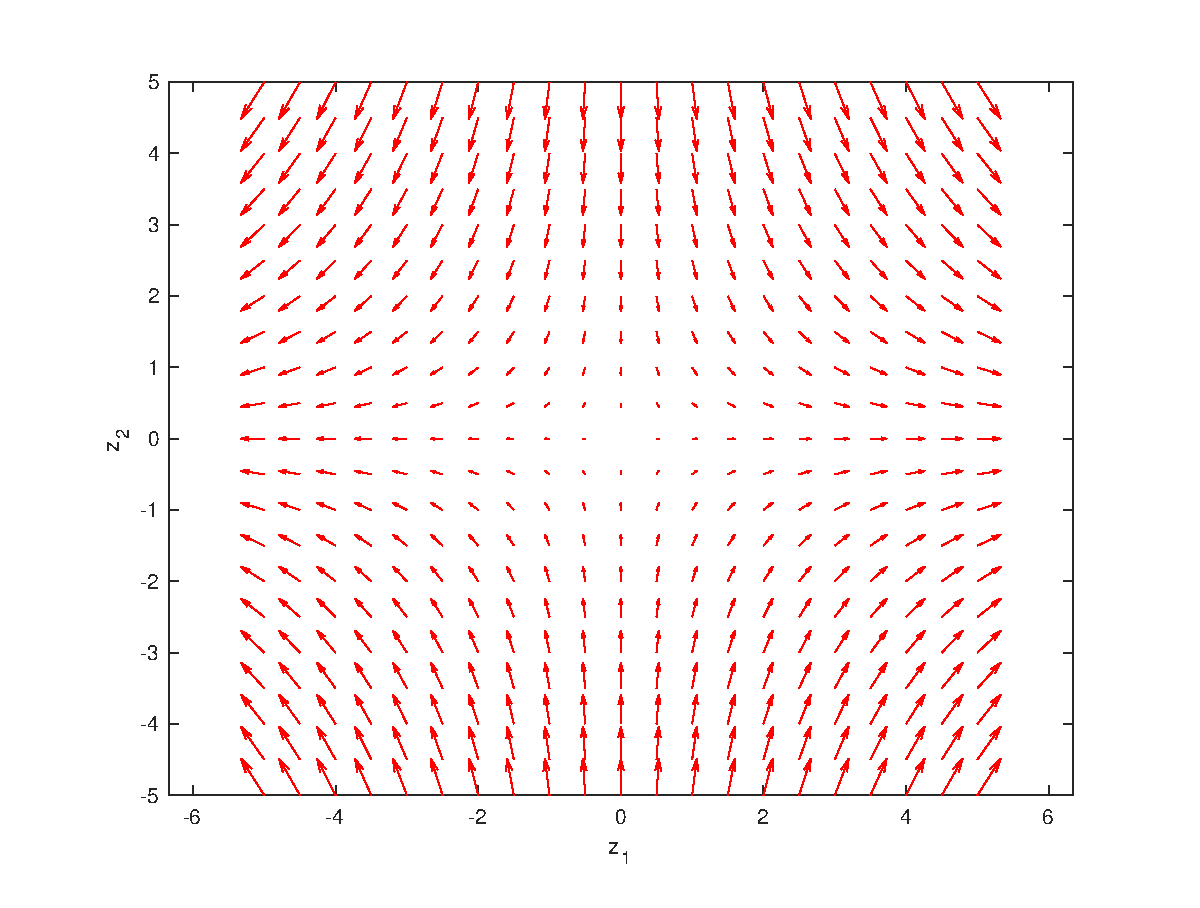
\includegraphics[width=0.5\textwidth]{images/chapter_1/phase_portrait_li.eps}
    \caption{Diagrama de fases en coordenadas modales.}
    \label{portrait_phase}
\end{figure}